\documentclass[tikz,border=10pt]{standalone}
\usepackage{amsmath,amssymb}
\usetikzlibrary{
  positioning,
  shapes.geometric,
  arrows.meta,
  backgrounds,
  fit,
  calc,
  decorations.pathreplacing
}

\begin{document}
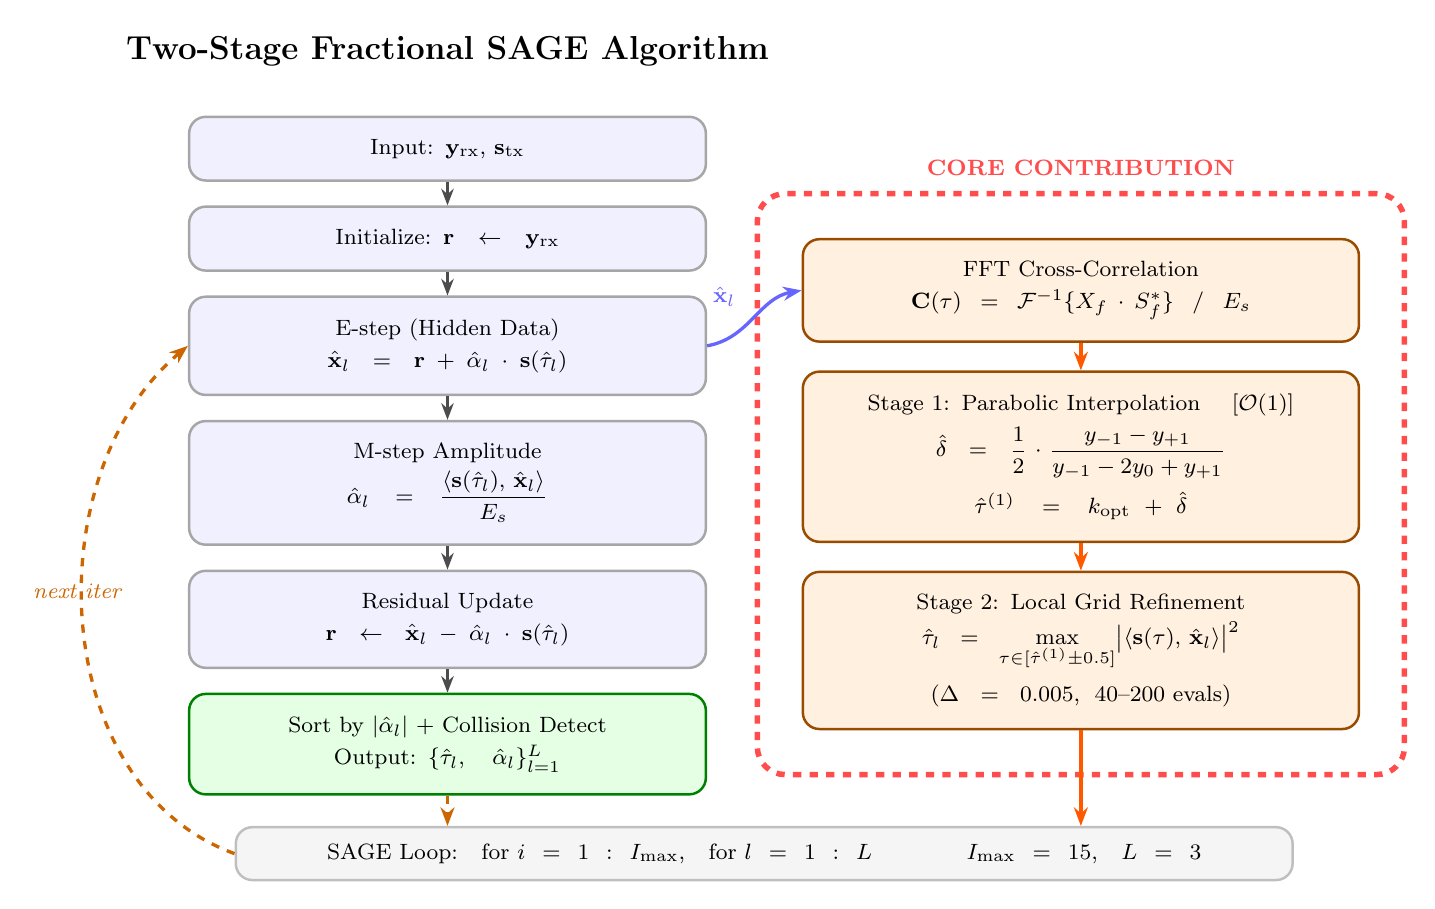
\begin{tikzpicture}[
  % ====== Box styles ======
  box_main/.style={
    draw=black!35, fill=blue!6, rounded corners=6pt,
    text width=6.0cm, align=center, inner sep=8pt,
    font=\footnotesize, line width=0.9pt
  },
  %
  box_core/.style={
    draw=orange!60!black, fill=orange!12, rounded corners=6pt,
    text width=6.5cm, align=center, inner sep=8pt,
    font=\footnotesize, line width=0.9pt
  },
  box_out/.style={
    draw=green!50!black, fill=green!10, rounded corners=6pt,
    text width=6.0cm, align=center, inner sep=8pt,
    font=\footnotesize, line width=0.9pt
  },
  box_loop/.style={
    draw=gray!50, fill=gray!8, rounded corners=6pt,
    text width=13.0cm, align=center, inner sep=6pt,
    font=\footnotesize, line width=0.9pt
  },
  %
  % ====== Arrow styles ======
  arr_black/.style={-{Stealth[scale=0.8]}, line width=1.0pt, black!70},
  arr_orange/.style={-{Stealth[scale=0.8]}, line width=1.2pt, orange!70!red},
  arr_blue/.style={-{Stealth[scale=0.8]}, line width=1.2pt, blue!60},
  arr_loop/.style={-{Stealth[scale=0.8]}, line width=1.2pt, orange!80!black, dashed},
  %
  % ====== Label style ======
  label_blue/.style={font=\footnotesize\itshape, blue!60, inner sep=2pt},
  label_loop/.style={font=\footnotesize\itshape, orange!80!black, inner sep=2pt},
]

% ================================================================
% TITLE
% ================================================================
\node[font=\large\bfseries, anchor=south] (title) at (0,0)
  {Two-Stage Fractional SAGE Algorithm};

% ================================================================
% LEFT COLUMN — Main SAGE loop (blue boxes)
% ================================================================
\node[box_main, below=0.5cm of title] (input)
  {Input: $\mathbf{y}_{\mathrm{rx}}$, $\mathbf{s}_{\mathrm{tx}}$};

\node[box_main, below=0.3cm of input] (init)
  {Initialize: $\mathbf{r} \leftarrow \mathbf{y}_{\mathrm{rx}}$};

\node[box_main, below=0.3cm of init] (estep)
  {E-step (Hidden Data)\\[2pt]
   $\hat{\mathbf{x}}_l = \mathbf{r} + \hat{\alpha}_l \cdot \mathbf{s}(\hat{\tau}_l)$};

\node[box_main, below=0.3cm of estep] (mstep)
  {M-step Amplitude\\[2pt]
   $\hat{\alpha}_l = \dfrac{\langle \mathbf{s}(\hat{\tau}_l),\,\hat{\mathbf{x}}_l \rangle}{E_s}$};

\node[box_main, below=0.3cm of mstep] (resid)
  {Residual Update\\[2pt]
   $\mathbf{r} \leftarrow \hat{\mathbf{x}}_l - \hat{\alpha}_l \cdot \mathbf{s}(\hat{\tau}_l)$};

\node[box_out, below=0.3cm of resid] (output)
  {Sort by $|\hat{\alpha}_l|$ + Collision Detect\\[2pt]
   Output: $\{\hat{\tau}_l,\;\hat{\alpha}_l\}_{l=1}^{L}$};

% ================================================================
% RIGHT COLUMN — Core contribution (orange boxes)
% ================================================================
\node[box_core, right=1.2cm of input, yshift=-1.8cm] (fft)
  {FFT Cross-Correlation\\[2pt]
   $\mathbf{C}(\tau) = \mathcal{F}^{-1}\{X_f \cdot S_f^*\}\;/\;E_s$};

\node[box_core, below=0.35cm of fft] (stage1)
  {Stage 1: Parabolic Interpolation \quad $[\mathcal{O}(1)]$\\[3pt]
   $\hat{\delta} = \dfrac{1}{2}\!\cdot\!\dfrac{y_{-1} - y_{+1}}{y_{-1} - 2y_0 + y_{+1}}$\\[4pt]
   $\hat{\tau}^{(1)} = k_{\mathrm{opt}} + \hat{\delta}$};

\node[box_core, below=0.35cm of stage1] (stage2)
  {Stage 2: Local Grid Refinement\\[2pt]
   $\hat{\tau}_l = \displaystyle\max_{\tau\in[\hat{\tau}^{(1)}\pm 0.5]}
   \bigl|\langle\mathbf{s}(\tau),\,\hat{\mathbf{x}}_l\rangle\bigr|^2$\\[4pt]
   ($\Delta = 0.005$,\; 40--200 evals)};

% ================================================================
% RED DASHED HIGHLIGHT RECTANGLE around core boxes
% ================================================================
\begin{scope}[on background layer]
\node[draw=red!70, line width=2.0pt, dashed, rounded corners=10pt,
      inner sep=16pt, fit=(fft)(stage1)(stage2)] (core_rect) {};
\end{scope}
\node[font=\bfseries\footnotesize, red!70, above=2pt of core_rect.north]
  {CORE CONTRIBUTION};

% ================================================================
% BOTTOM GRAY LOOP BOX — centered between both columns
% ================================================================
% Compute center between left (output) and right (stage2) columns
\coordinate (col_center) at ($(output.south)!0.5!(stage2.south)$);
\node[box_loop, below=0.8cm of col_center] (loopbox)
  {SAGE Loop:\quad for $i = 1 : I_{\max}$,\quad for $l = 1 : L$\hspace{1.2cm}$I_{\max} = 15$,\quad $L = 3$};

% ================================================================
% ARROWS — Left column (vertical, black)
% ================================================================
\draw[arr_black] (input.south)  -- (init.north);
\draw[arr_black] (init.south)   -- (estep.north);
\draw[arr_black] (estep.south)  -- (mstep.north);
\draw[arr_black] (mstep.south)  -- (resid.north);
\draw[arr_black] (resid.south)  -- (output.north);

% ================================================================
% ARROWS — Right column (vertical, orange)
% ================================================================
\draw[arr_orange] (fft.south)    -- (stage1.north);
\draw[arr_orange] (stage1.south) -- (stage2.north);

% ================================================================
% CROSS ARROW — E-step -> FFT (blue, angled)
% ================================================================
\draw[arr_blue] (estep.east) to[out=10, in=190]
  node[label_blue, pos=0.45, above left=4pt] {$\hat{\mathbf{x}}_l$}
  (fft.west);

% ================================================================
% LOOP ARROWS — both columns → straight down → loop box
% ================================================================
% Left: green output → loop box (straight down)
\draw[arr_loop] (output.south) -- (output.south |- loopbox.north);

% Right: Stage 2 → loop box (straight down)
\draw[arr_orange] (stage2.south) -- (stage2.south |- loopbox.north);

% Loop box → E-step (gentle curve back for next iteration)
\draw[arr_loop]
  (loopbox.west) to[out=160, in=220]
  node[label_loop, pos=0.55, xshift=-2pt] {next iter}
  (estep.west);

\end{tikzpicture}
\end{document}
